\documentclass[journal,compsoc]{IEEEtran}
\usepackage{amsmath,amssymb}
\usepackage{tikz}
\usetikzlibrary{arrows.meta,positioning,shapes.geometric,fit,calc,backgrounds}
\usepackage{xcolor}

% Color definitions
\definecolor{tierclient}{RGB}{236,244,252}
\definecolor{tierclientborder}{RGB}{41,128,185}
\definecolor{tiergate}{RGB}{254,249,238}
\definecolor{tiergateborder}{RGB}{214,137,16}
\definecolor{tierfast}{RGB}{247,243,252}
\definecolor{tierfastborder}{RGB}{142,68,173}
\definecolor{tierdb}{RGB}{237,247,242}
\definecolor{tierdbborder}{RGB}{39,174,96}

\tikzset{
  cnode/.style={draw=#1, fill=white, rounded corners=3pt, line width=0.7pt, align=center},
  dnode/.style={draw=#1, cylinder, shape border rotate=90, aspect=0.25, fill=white, line width=0.7pt, align=center},
  arrow/.style={-{Stealth[length=2.2mm,width=1.5mm]}, line width=0.8pt, draw=black!75},
  darrow/.style={{Stealth[length=2mm,width=1.3mm]}-{Stealth[length=2mm,width=1.3mm]}, line width=0.8pt, draw=black!75},
  labeltext/.style={font=\tiny\bfseries, text=black!80},
  qnode/.style={draw=black!70, fill=black!5, rounded corners=3pt, line width=0.7pt, align=center, font=\scriptsize},
  snode/.style={draw=#1, fill=white, rounded corners=2.5pt, line width=0.6pt, align=center, font=\scriptsize},
  fnode/.style={draw=#1, fill=#1!12, rounded corners=3pt, line width=0.7pt, align=center, font=\scriptsize},
  farrow/.style={-{Stealth[length=2mm,width=1.3mm]}, line width=0.7pt, draw=black!75},
  agentnode/.style={draw=tierfastborder, fill=white, rounded corners=2.5pt, line width=0.6pt, align=center, font=\tiny, text width=16.5mm, minimum height=6.5mm},
  startnode/.style={draw=black!70, fill=black!6, rounded corners=2.5pt, line width=0.7pt, align=center, font=\tiny\bfseries, text width=12mm, minimum height=6.5mm},
  endnode/.style={draw=tierdbborder, fill=tierdb!40, rounded corners=2.5pt, line width=0.7pt, align=center, font=\tiny\bfseries, text width=12mm, minimum height=6.5mm},
  pnode/.style={draw=#1, fill=white, rounded corners=2.5pt, line width=0.6pt, align=center, font=\tiny, text width=22.5mm, minimum height=7mm}
}

\begin{document}

% =========================================================================
% FIGURE 1: Two-column High-Level Architecture
% =========================================================================
\begin{figure*}
\centering
\resizebox{0.96\textwidth}{!}{%
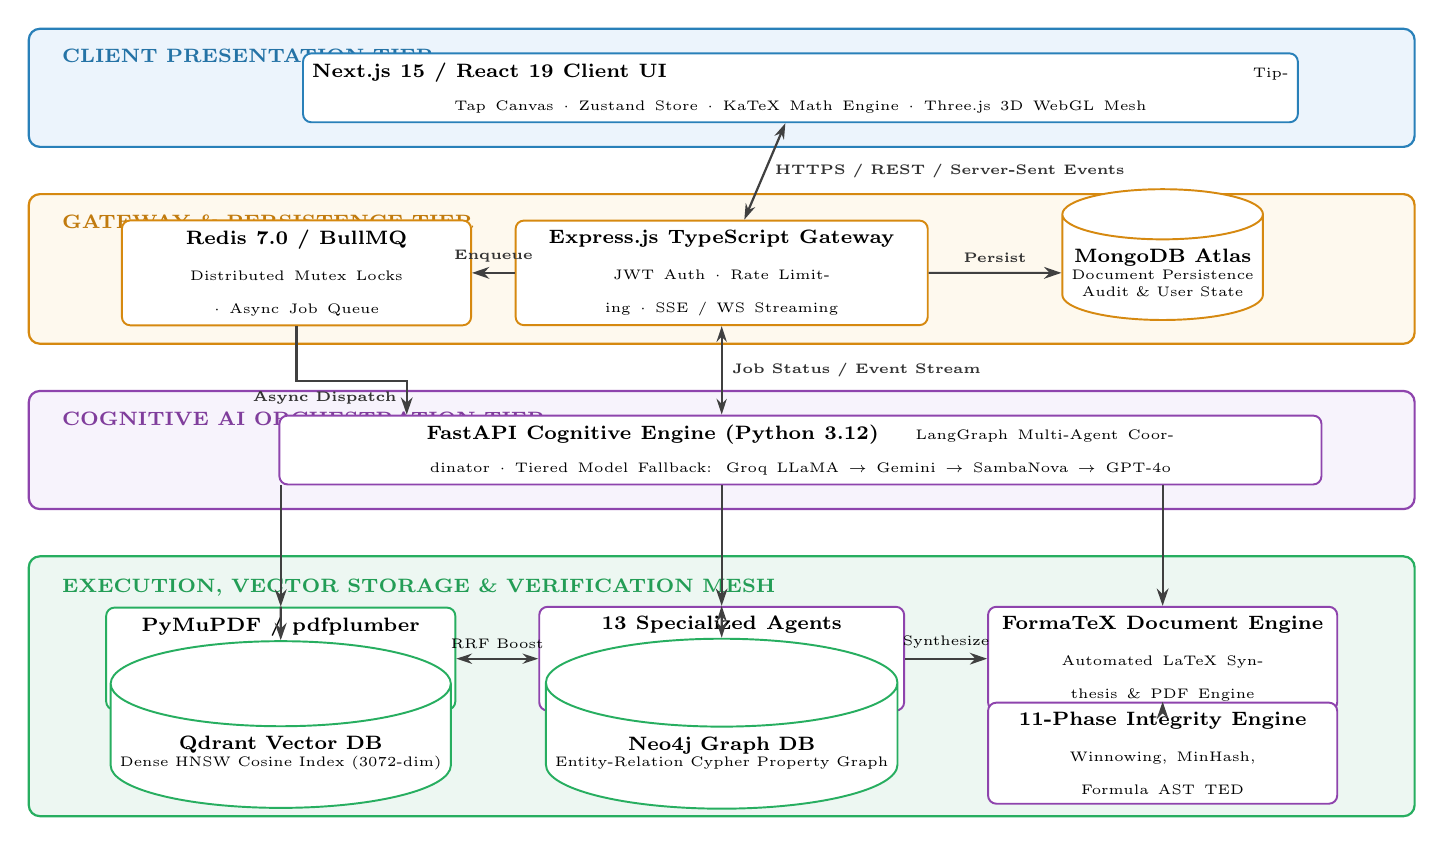
\begin{tikzpicture}[x=1mm, y=1mm]

% --- TIER 1: CLIENT TIER ---
\draw[rounded corners=4pt, fill=tierclient, draw=tierclientborder, line width=0.8pt] (-88, 54) rectangle (88, 69);
\node[anchor=west, font=\scriptsize\bfseries, text=tierclientborder!90!black] at (-85, 65.5) {CLIENT PRESENTATION TIER};
\node[cnode=tierclientborder, text width=124mm, minimum height=7.5mm] (client) at (10, 61.5) {
  \textbf{\scriptsize Next.js 15 / React 19 Client UI} \hfill \tiny TipTap Canvas $\cdot$ Zustand Store $\cdot$ KaTeX Math Engine $\cdot$ Three.js 3D WebGL Mesh
};

% --- TIER 2: GATEWAY & QUEUING TIER ---
\draw[rounded corners=4pt, fill=tiergate, draw=tiergateborder, line width=0.8pt] (-88, 29) rectangle (88, 48);
\node[anchor=west, font=\scriptsize\bfseries, text=tiergateborder!90!black] at (-85, 44.5) {GATEWAY \& PERSISTENCE TIER};

\node[cnode=tiergateborder, text width=42mm, minimum height=10mm] (redis) at (-54, 38) {
  \textbf{\scriptsize Redis 7.0 / BullMQ}\\[1pt]
  \tiny Distributed Mutex Locks $\cdot$ Async Job Queue
};

\node[cnode=tiergateborder, text width=50mm, minimum height=10mm] (gateway) at (0, 38) {
  \textbf{\scriptsize Express.js TypeScript Gateway}\\[1pt]
  \tiny JWT Auth $\cdot$ Rate Limiting $\cdot$ SSE / WS Streaming
};

\node[dnode=tiergateborder, minimum width=24mm, minimum height=10mm, font=\tiny] (mongo) at (56, 38) {
  \textbf{\scriptsize MongoDB Atlas}\\
  Document Persistence\\
  Audit \& User State
};

% --- TIER 3: COGNITIVE ORCHESTRATION TIER ---
\draw[rounded corners=4pt, fill=tierfast, draw=tierfastborder, line width=0.8pt] (-88, 8) rectangle (88, 23);
\node[anchor=west, font=\scriptsize\bfseries, text=tierfastborder!90!black] at (-85, 19.5) {COGNITIVE AI ORCHESTRATION TIER};

\node[cnode=tierfastborder, text width=130mm, minimum height=8.5mm] (fastapi) at (10, 15.5) {
  \textbf{\scriptsize FastAPI Cognitive Engine (Python 3.12)} \quad
  \tiny LangGraph Multi-Agent Coordinator $\cdot$ Tiered Model Fallback: Groq LLaMA $\to$ Gemini $\to$ SambaNova $\to$ GPT-4o
};

% --- TIER 4: STORAGE & VERIFICATION MESH ---
\draw[rounded corners=4pt, fill=tierdb, draw=tierdbborder, line width=0.8pt] (-88, -31) rectangle (88, 2);
\node[anchor=west, font=\scriptsize\bfseries, text=tierdbborder!90!black] at (-85, -2) {EXECUTION, VECTOR STORAGE \& VERIFICATION MESH};

% Column 1: Ingestion & Vector
\node[cnode=tierdbborder, text width=42mm, minimum height=9.5mm] (ingest) at (-56, -11) {
  \textbf{\scriptsize PyMuPDF / pdfplumber}\\[1pt]
  \tiny Layout-Aware Ingestion \& Math Extraction
};
\node[dnode=tierdbborder, minimum width=26mm, minimum height=9.5mm, font=\tiny] (qdrant) at (-56, -23) {
  \textbf{\scriptsize Qdrant Vector DB}\\
  Dense HNSW Cosine Index (3072-dim)
};

% Column 2: Agents & Graph Mesh
\node[cnode=tierfastborder, text width=44mm, minimum height=9.5mm] (agents) at (0, -11) {
  \textbf{\scriptsize 13 Specialized Agents}\\[1pt]
  \tiny Planner, Researcher, Fact-Check, Reviewer...
};
\node[dnode=tierdbborder, minimum width=26mm, minimum height=9.5mm, font=\tiny] (neo4j) at (0, -23) {
  \textbf{\scriptsize Neo4j Graph DB}\\
  Entity-Relation Cypher Property Graph
};

% Column 3: FormaTeX & Integrity
\node[cnode=tierfastborder, text width=42mm, minimum height=9.5mm] (formatex) at (56, -11) {
  \textbf{\scriptsize FormaTeX Document Engine}\\[1pt]
  \tiny Automated LaTeX Synthesis \& PDF Engine
};
\node[cnode=tierfastborder, text width=42mm, minimum height=9.5mm] (integrity) at (56, -23) {
  \textbf{\scriptsize 11-Phase Integrity Engine}\\[1pt]
  \tiny Winnowing, MinHash, Formula AST TED
};

% ARROWS
\draw[darrow] (client) -- node[right, labeltext] {HTTPS / REST / Server-Sent Events} (gateway);
\draw[arrow] (gateway) -- node[above, labeltext] {Enqueue} (redis);
\draw[arrow] (gateway) -- node[above, labeltext] {Persist} (mongo);

\draw[arrow] (redis.south) -- ++(0,-7) -| node[near end, left, labeltext] {Async Dispatch} (-40, 20);
\draw[darrow] (gateway.south) -- node[right, labeltext] {Job Status / Event Stream} (0, 20);

\draw[arrow] (-56, 11) -- (ingest);
\draw[arrow] (0, 11) -- (agents);
\draw[arrow] (56, 11) -- (formatex);

\draw[arrow] (ingest) -- (qdrant);
\draw[darrow] (agents) -- (neo4j);
\draw[darrow] (agents.west) -- node[above, font=\tiny] {RRF Boost} (ingest.east);
\draw[arrow] (agents.east) -- node[above, font=\tiny] {Synthesize} (formatex.west);
\draw[arrow] (formatex) -- (integrity);

\end{tikzpicture}}
\caption{Distributed architecture of ResearcherGPT across client, gateway, cognitive orchestration, and storage mesh tiers.}
\label{fig:architecture}
\end{figure*}

\newpage

% =========================================================================
% FIGURE 2: Tri-Hybrid Retrieval Pipeline
% =========================================================================
\begin{figure}[!b]
\centering
\resizebox{0.98\columnwidth}{!}{%
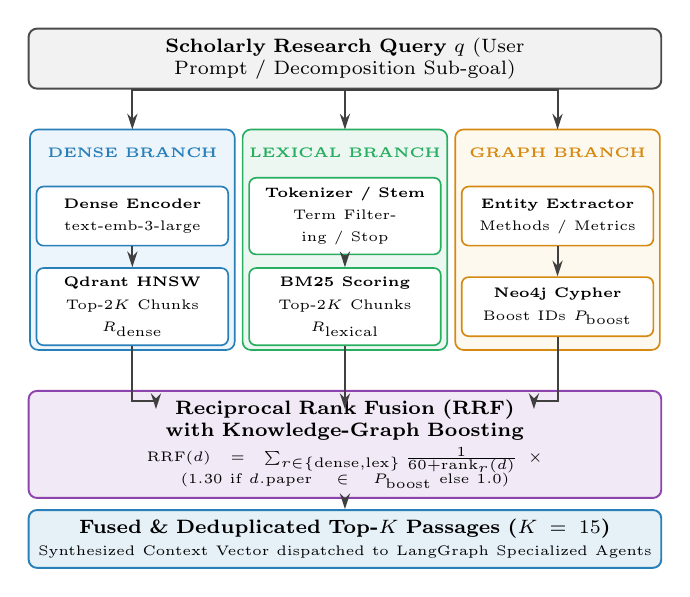
\begin{tikzpicture}[x=1mm, y=1mm]

% Top: Query Node
\node[qnode, text width=78mm, minimum height=6.5mm] (query) at (0, 48) {
  \textbf{Scholarly Research Query $q$} (User Prompt / Decomposition Sub-goal)
};

% Branch 1: Dense Semantic Branch (Left, x = -27)
\draw[rounded corners=3pt, fill=tierclient, draw=tierclientborder, line width=0.6pt] (-40, 11) rectangle (-14, 39);
\node[font=\tiny\bfseries, text=tierclientborder] at (-27, 36) {DENSE BRANCH};
\node[snode=tierclientborder, text width=22mm, minimum height=7.5mm] (d1) at (-27, 28) {
  \tiny\textbf{Dense Encoder}\\
  \tiny text-emb-3-large
};
\node[snode=tierclientborder, text width=22mm, minimum height=7.5mm] (d2) at (-27, 16.5) {
  \tiny\textbf{Qdrant HNSW}\\
  \tiny Top-$2K$ Chunks $R_{\mathrm{dense}}$
};
\draw[farrow] (d1) -- (d2);

% Branch 2: Sparse Lexical Branch (Center, x = 0)
\draw[rounded corners=3pt, fill=tierdb, draw=tierdbborder, line width=0.6pt] (-13, 11) rectangle (13, 39);
\node[font=\tiny\bfseries, text=tierdbborder] at (0, 36) {LEXICAL BRANCH};
\node[snode=tierdbborder, text width=22mm, minimum height=7.5mm] (l1) at (0, 28) {
  \tiny\textbf{Tokenizer / Stem}\\
  \tiny Term Filtering / Stop
};
\node[snode=tierdbborder, text width=22mm, minimum height=7.5mm] (l2) at (0, 16.5) {
  \tiny\textbf{BM25 Scoring}\\
  \tiny Top-$2K$ Chunks $R_{\mathrm{lexical}}$
};
\draw[farrow] (l1) -- (l2);

% Branch 3: Knowledge Graph Branch (Right, x = 27)
\draw[rounded corners=3pt, fill=tiergate, draw=tiergateborder, line width=0.6pt] (14, 11) rectangle (40, 39);
\node[font=\tiny\bfseries, text=tiergateborder] at (27, 36) {GRAPH BRANCH};
\node[snode=tiergateborder, text width=22mm, minimum height=7.5mm] (g1) at (27, 28) {
  \tiny\textbf{Entity Extractor}\\
  \tiny Methods / Metrics
};
\node[snode=tiergateborder, text width=22mm, minimum height=7.5mm] (g2) at (27, 16.5) {
  \tiny\textbf{Neo4j Cypher}\\
  \tiny Boost IDs $P_{\mathrm{boost}}$
};
\draw[farrow] (g1) -- (g2);

% Query dispatch arrows
\draw[farrow] (query.south) -| (-27, 39);
\draw[farrow] (query.south) -- (0, 39);
\draw[farrow] (query.south) -| (27, 39);

% Fusion Layer
\node[fnode=tierfastborder, text width=78mm, minimum height=8.5mm] (rrf) at (0, -1) {
  \textbf{Reciprocal Rank Fusion (RRF) with Knowledge-Graph Boosting}\\[1pt]
  \tiny $\mathrm{RRF}(d) = \sum_{r \in \{\mathrm{dense}, \mathrm{lex}\}} \frac{1}{60 + \mathrm{rank}_r(d)} \times (1.30 \text{ if } d.\mathrm{paper} \in P_{\mathrm{boost}} \text{ else } 1.0)$
};

% Convergence arrows into RRF
\draw[farrow] (d2.south) |- (-24, 4.5) -- (-24, 3.5);
\draw[farrow] (l2.south) -- (0, 3.5);
\draw[farrow] (g2.south) |- (24, 4.5) -- (24, 3.5);

% Output Node
\node[fnode=tierclientborder, text width=78mm, minimum height=6.5mm] (out) at (0, -13) {
  \textbf{Fused \& Deduplicated Top-$K$ Passages ($K=15$)}\\
  \tiny Synthesized Context Vector dispatched to LangGraph Specialized Agents
};
\draw[farrow, line width=0.9pt] (rrf) -- (out);

\end{tikzpicture}}
\caption{Tri-hybrid retrieval pipeline combining dense vector embeddings, BM25 lexical scoring, and Neo4j graph boosting via Reciprocal Rank Fusion.}
\label{fig:retrieval}
\end{figure}

\newpage

% =========================================================================
% FIGURE 3: Multi-Agent Workflow
% =========================================================================
\begin{figure}[!t]
\centering
\resizebox{0.98\columnwidth}{!}{%
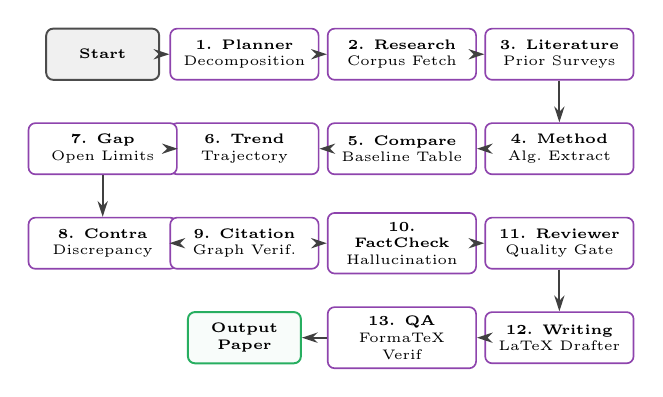
\begin{tikzpicture}[x=1mm, y=1mm]

% ROW 1: Planning & Discovery (Left to Right)
\node[startnode] (start) at (-34.5, 30) {Start};
\node[agentnode] (planner) at (-16.5, 30) {\textbf{1. Planner}\\Decomposition};
\node[agentnode] (researcher) at (3.5, 30) {\textbf{2. Research}\\Corpus Fetch};
\node[agentnode] (lit) at (23.5, 30) {\textbf{3. Literature}\\Prior Surveys};

\draw[farrow] (start) -- (planner);
\draw[farrow] (planner) -- (researcher);
\draw[farrow] (researcher) -- (lit);

% Turn 1: lit -> meth (direct downward vertical arrow at right margin)
\node[agentnode] (meth) at (23.5, 18) {\textbf{4. Method}\\Alg.\ Extract};
\node[agentnode] (comp) at (3.5, 18) {\textbf{5. Compare}\\Baseline Table};
\node[agentnode] (trend) at (-16.5, 18) {\textbf{6. Trend}\\Trajectory};
\node[agentnode] (gap) at (-34.5, 18) {\textbf{7. Gap}\\Open Limits};

\draw[farrow] (lit) -- (meth);
\draw[farrow] (meth) -- (comp);
\draw[farrow] (comp) -- (trend);
\draw[farrow] (trend) -- (gap);

% Turn 2: gap -> contra (direct downward vertical arrow at left margin)
\node[agentnode] (contra) at (-34.5, 6) {\textbf{8. Contra}\\Discrepancy};
\node[agentnode] (cite) at (-16.5, 6) {\textbf{9. Citation}\\Graph Verif.};
\node[agentnode] (fact) at (3.5, 6) {\textbf{10. FactCheck}\\Hallucination};
\node[agentnode] (rev) at (23.5, 6) {\textbf{11. Reviewer}\\Quality Gate};

\draw[farrow] (gap) -- (contra);
\draw[farrow] (contra) -- (cite);
\draw[farrow] (cite) -- (fact);
\draw[farrow] (fact) -- (rev);

% Turn 3: rev -> write (direct downward vertical arrow at right margin)
\node[agentnode] (write) at (23.5, -6) {\textbf{12. Writing}\\LaTeX Drafter};
\node[agentnode] (qa) at (3.5, -6) {\textbf{13. QA}\\FormaTeX Verif};
\node[endnode] (end) at (-16.5, -6) {Output\\Paper};

\draw[farrow] (rev) -- (write);
\draw[farrow] (write) -- (qa);
\draw[farrow] (qa) -- (end);

\end{tikzpicture}}
\caption{Principal execution path through the thirteen-agent research synthesis workflow.}
\label{fig:agents}
\end{figure}

\newpage

% =========================================================================
% FIGURE 4: Eleven Phases of Academic Integrity Verification
% =========================================================================
\begin{figure}[!t]
\centering
\resizebox{0.98\columnwidth}{!}{%
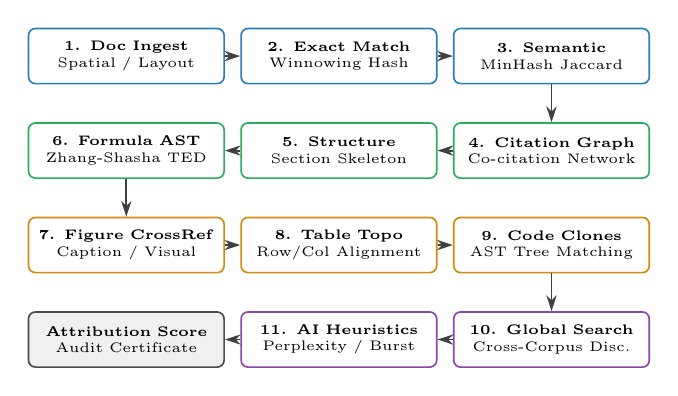
\begin{tikzpicture}[x=1mm, y=1mm]

% ROW 1 (T1: Lexical & Semantic) Left to Right
\node[pnode=tierclientborder] (p1) at (-27, 24) {\textbf{1. Doc Ingest}\\Spatial / Layout};
\node[pnode=tierclientborder] (p2) at (0, 24) {\textbf{2. Exact Match}\\Winnowing Hash};
\node[pnode=tierclientborder] (p3) at (27, 24) {\textbf{3. Semantic}\\MinHash Jaccard};

\draw[farrow] (p1) -- (p2);
\draw[farrow] (p2) -- (p3);

% Turn 1: p3 -> p4 (downward at right)
\node[pnode=tierdbborder] (p4) at (27, 12) {\textbf{4. Citation Graph}\\Co-citation Network};
\node[pnode=tierdbborder] (p5) at (0, 12) {\textbf{5. Structure}\\Section Skeleton};
\node[pnode=tierdbborder] (p6) at (-27, 12) {\textbf{6. Formula AST}\\Zhang-Shasha TED};

\draw[farrow] (p3) -- (p4);
\draw[farrow] (p4) -- (p5);
\draw[farrow] (p5) -- (p6);

% Turn 2: p6 -> p7 (downward at left)
\node[pnode=tiergateborder] (p7) at (-27, 0) {\textbf{7. Figure CrossRef}\\Caption / Visual};
\node[pnode=tiergateborder] (p8) at (0, 0) {\textbf{8. Table Topo}\\Row/Col Alignment};
\node[pnode=tiergateborder] (p9) at (27, 0) {\textbf{9. Code Clones}\\AST Tree Matching};

\draw[farrow] (p6) -- (p7);
\draw[farrow] (p7) -- (p8);
\draw[farrow] (p8) -- (p9);

% Turn 3: p9 -> p10 (downward at right)
\node[pnode=tierfastborder] (p10) at (27, -12) {\textbf{10. Global Search}\\Cross-Corpus Disc.};
\node[pnode=tierfastborder] (p11) at (0, -12) {\textbf{11. AI Heuristics}\\Perplexity / Burst};
\node[pnode=black!70, fill=black!6] (pout) at (-27, -12) {\textbf{Attribution Score}\\Audit Certificate};

\draw[farrow] (p9) -- (p10);
\draw[farrow] (p10) -- (p11);
\draw[farrow] (p11) -- (pout);

\end{tikzpicture}}
\caption{Eleven phases of the academic-integrity verification and attribution engine.}
\label{fig:integrity}
\end{figure}

\end{document}
